\documentclass{article}%
\usepackage[T1]{fontenc}%
\usepackage[utf8]{inputenc}%
\usepackage{lmodern}%
\usepackage{textcomp}%
\usepackage{lastpage}%
\usepackage{graphicx}%
%
\title{Harry Potter}%
\author{JK }%
\date{\today}%
%
\begin{document}%
\normalsize%


\begin{figure}[h!]%
\centering%
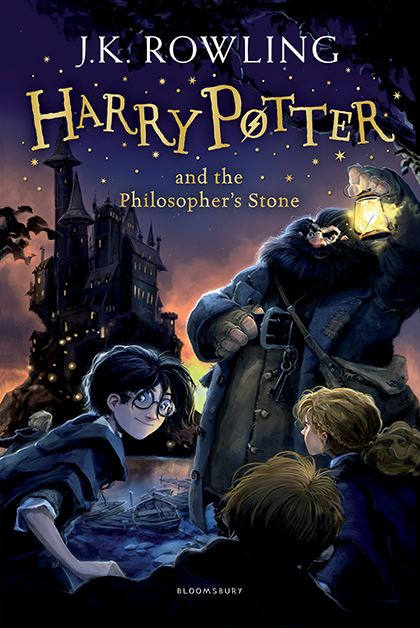
\includegraphics[width=300px]{C:/Users/sastr/Documents/ComputerScience/FinalProject/harryPotter.jpg}%
\end{figure}

%
\maketitle%


\begin{figure}[h!]%
\centering%
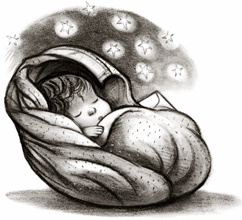
\includegraphics[width=200px]{C:/Users/sastr/Documents/ComputerScience/FinalProject/baby.jpg}%
\end{figure}

%

\newline%
Harry Potter and the Sorcerer's Stone
\newline%
CHAPTER ONE
\newline%
THE BOY WHO LIVED
\newline%

\newline%
Mr. and Mrs. Dursley, of number four, Privet Drive, were proud to say
\newline%
that they were perfectly normal, thank you very much. They were the last
\newline%
people you'd expect to be involved in anything strange or mysterious,
\newline%
because they just didn't hold with such nonsense.
\newline%
Mr. Dursley was the director of a firm called Grunnings, which made
\newline%
drills. He was a big, beefy man with hardly any neck, although he did
\newline%
have a very large mustache. Mrs. Dursley was thin and blonde and had
\newline%
nearly twice the usual amount of neck, which came in very useful as she
\newline%
spent so much of her time craning over garden fences, spying on the
\newline%
neighbors. The Dursleys had a small son called Dudley and in their
\newline%
opinion there was no finer boy anywhere.
\newline%
The Dursleys had everything they wanted, but they also had a secret, and
\newline%
their greatest fear was that somebody would discover it. They didn't
\newline%
think they could bear it if anyone found out about the Potters. Mrs.
\newline%
Potter was Mrs. Dursley's sister, but they hadn't met for several years;
\newline%
in fact, Mrs. Dursley pretended she didn't have a sister, because her
\newline%
sister and her good{-}for{-}nothing husband were as unDursleyish as it was
\newline%
possible to be. The Dursleys shuddered to think what the neighbors would
\newline%
say if the Potters arrived in the street. The Dursleys knew that the
\newline%
Potters had a small son, too, but they had never even seen him. This boy
\newline%
was another good reason for keeping the Potters away; they didn't want
\newline%
Dudley mixing with a child like that.
\newline%
When Mr. and Mrs. Dursley woke up on the dull, gray Tuesday our story
\newline%
starts, there was nothing about the cloudy sky outside to suggest that
\newline%
strange and mysterious things would soon be happening all over the
\newline%
country. Mr. Dursley hummed as he picked out his most boring tie for
\newline%
work, and Mrs. Dursley gossiped away happily as she wrestled a screaming
\newline%
Dudley into his high chair.
\newline%
None of them noticed a large, tawny owl flutter past the window.
\newline%
At half past eight, Mr. Dursley picked up his briefcase, pecked Mrs.
\newline%
Dursley on the cheek, and tried to kiss Dudley good{-}bye but missed,
\newline%
2
\newline%
because Dudley was now having a tantrum and throwing his cereal at the
\newline%
walls. "Little tyke," chortled Mr. Dursley as he left the house. He got
\newline%
into his car and backed out of number four's drive.
\newline%
It was on the corner of the street that he noticed the first sign of
\newline%
something peculiar {-}{-} a cat reading a map. For a second, Mr. Dursley
\newline%
didn't realize what he had seen {-}{-} then he jerked his head around to
\newline%
look again. There was a tabby cat standing on the corner of Privet
\newline%
Drive, but there wasn't a map in sight. What could he have been thinking
\newline%
of? It must have been a trick of the light. Mr. Dursley blinked and
\newline%
stared at the cat. It stared back. As Mr. Dursley drove around the
\newline%
corner and up the road, he watched the cat in his mirror. It was now
\newline%
reading the sign that said Privet Drive {-}{-} no, looking at the sign; cats
\newline%
couldn't read maps or signs. Mr. Dursley gave himself a little shake and
\newline%
put the cat out of his mind. As he drove toward town he thought of
\newline%
nothing except a large order of drills he was hoping to get that day.
\newline%
But on the edge of town, drills were driven out of his mind by something
\newline%
else. As he sat in the usual morning traffic jam, he couldn't help
\newline%
noticing that there seemed to be a lot of strangely dressed people
\newline%
about. People in cloaks. Mr. Dursley couldn't bear people who dressed in
\newline%
funny clothes {-}{-} the getups you saw on young people! He supposed this
\newline%
was some stupid new fashion. He drummed his fingers on the steering
\newline%
wheel and his eyes fell on a huddle of these weirdos standing quite
\newline%
close by. They were whispering excitedly together. Mr. Dursley was
\newline%
enraged to see that a couple of them weren't young at all; why, that man
\newline%
had to be older than he was, and wearing an emerald{-}green cloak! The
\newline%
nerve of him! But then it struck Mr. Dursley that this was probably some
\newline%
silly stunt {-}{-} these people were obviously collecting for something...
\newline%
yes, that would be it. The traffic moved on and a few minutes later, Mr
\newline%
3
\newline%
He'd forgotten all about the people in cloaks until he passed a group of
\newline%
them next to the baker's. He eyed them angrily as he passed. He didn't
\newline%
know why, but they made him uneasy. This bunch were whispering
\newline%
excitedly, too, and he couldn't see a single collecting tin. It was on
\newline%
his way back past them, clutching a large doughnut in a bag, that he
\newline%
caught a few words of what they were saying.
\newline%
"The Potters, that's right, that's what I heard yes, their son, Harry"
\newline%
Mr. Dursley stopped dead. Fear flooded him. He looked back at the
\newline%
whisperers as if he wanted to say something to them, but thought better
\newline%
of it.
\newline%
He dashed back across the road, hurried up to his office, snapped at his
\newline%
secretary not to disturb him, seized his telephone, and had almost
\newline%
finished dialing his home number when he changed his mind. He put the
\newline%
receiver back down and stroked his mustache, thinking... no, he was
\newline%
being stupid. Potter wasn't such an unusual name. He was sure there were
\newline%
lots of people called Potter who had a son called Harry. Come to think
\newline%
of it, he wasn't even sure his nephew was called Harry. He'd never even
\newline%
seen the boy. It might have been Harvey. Or Harold. There was no point
\newline%
in worrying Mrs. Dursley; she always got so upset at any mention of her
\newline%
sister. He didn't blame her {-}{-} if he'd had a sister like that... but all
\newline%
the same, those people in cloaks...
\newline%
He found it a lot harder to concentrate on drills that afternoon and
\newline%
when he left the building at five o'clock, he was still so worried that
\newline%
he walked straight into someone just outside the door.
\newline%
"Sorry," he grunted, as the tiny old man stumbled and almost fell. It
\newline%
was a few seconds before Mr. Dursley realized that the man was wearing a
\newline%
violet cloak. He didn't seem at all upset at being almost knocked to the
\newline%
ground. On the contrary, his face split into a wide smile and he said in
\newline%
a squeaky voice that made passersby stare, "Don't be sorry, my dear sir,
\newline%
for nothing could upset me today! Rejoice, for You{-}Know{-}Who has gone at
\newline%
last! Even Muggles like yourself should be celebrating, this happy,
\newline%
happy day!"
\newline%
And the old man hugged Mr. Dursley around the middle and walked off.
\newline%
Mr. Dursley stood rooted to the spot. He had been hugged by a complete
\newline%
stranger. He also thought he had been called a Muggle, whatever that
\newline%
was. He was rattled. He hurried to his car and set off for home, hoping
\newline%
4
\newline%
he was imagining things, which he had never hoped before, because he
\newline%
didn't approve of imagination.
\newline%
As he pulled into the driveway of number four, the first thing he saw {-}{-}
\newline%
and it didn't improve his mood {-}{-} was the tabby cat he'd spotted that
\newline%
morning. It was now sitting on his garden wall. He was sure it was the
\newline%
same one; it had the same markings around its eyes.
\newline%
"Shoo!" said Mr. Dursley loudly. The cat didn't move. It just gave him a
\newline%
stern look. Was this normal cat behavior? Mr. Dursley wondered. Trying
\newline%
to pull himself together, he let himself into the house. He was still
\newline%
determined not to mention anything to his wife.
\newline%
Mrs. Dursley had had a nice, normal day. She told him over dinner all
\newline%
about Mrs. Next Door's problems with her daughter and how Dudley had
\newline%
learned a new word ("Won't!"). Mr. Dursley tried to act normally. Whe
\newline%
5
\newline%
As he had expected, Mrs. Dursley looked shocked and angry. After all,
\newline%
they normally pretended she didn't have a sister.
\newline%
"No," she said sharply. "Why?"
\newline%
"Funny stuff on the news," Mr. Dursley mumbled. "Owls... shooting
\newline%
stars... and there were a lot of funny{-}looking people in town today..."
\newline%
"So?" snapped Mrs. Dursley.
\newline%
"Well, I just thought... maybe... it was something to do with... you
\newline%
know... her crowd."
\newline%
Mrs. Dursley sipped her tea through pursed lips. Mr. Dursley wondered
\newline%
whether he dared tell her he'd heard the name "Potter." He decided he
\newline%
didn't dare. Instead he said, as casually as he could, "Their son {-}{-}
\newline%
he'd be about Dudley's age now, wouldn't he?"
\newline%
"I suppose so," said Mrs. Dursley stiffly.
\newline%
"What's his name again? Howard, isn't it?"
\newline%
"Harry. Nasty, common name, if you ask me."
\newline%
"Oh, yes," said Mr. Dursley, his heart sinking horribly. "Yes, I quite
\newline%
agree."
\newline%
He didn't say another word on the subject as they went upstairs to bed.
\newline%
While Mrs. Dursley was in the bathroom, Mr. Dursley crept to the bedroom
\newline%
window and peered down into the front garden. The cat was still there.
\newline%
It was staring down Privet Drive as though it were waiting for
\newline%
something.
\newline%
Was he imagining things? Could all this have anything to do with the
\newline%
Potters? If it did... if it got out that they were related to a pair of
\newline%
{-}{-} well, he didn't think he could bear it.
\newline%
The Dursleys got into bed. Mrs. Dursley fell asleep quickly but Mr.
\newline%
Dursley lay awake, turning it all over in his mind. His last, comforting
\newline%
thought before he fell asleep was that even if the Potters were
\newline%
involved, there was no reason for them to come near him and Mrs.
\newline%
Dursley. The Potters knew very well what he and Petunia thought about
\newline%
6
\newline%
them and their kind.... He couldn't see how he and Petunia could get
\newline%
mixed up in anything that might be going on {-}{-} he yawned and turned over
\newline%
{-}{-} it couldn't affect them....
\newline%
How very wrong he was.
\newline%
Mr. Dursley might have been drifting into an uneasy sleep, but the cat
\newline%
on the wall outside was showing no sign of sleepiness. It was sitting as
\newline%
still as a statue, its eyes fixed unblinkingly on the far corner of
\newline%
Privet Drive. It didn't so much as quiver when a car door slammed on the
\newline%
next street, nor when two owls swooped overhead. In fact, it was nearly
\newline%
midnight before the cat moved at all.
\newline%
A man appeared on the corner the cat had been watching, appeared so
\newline%
suddenly and silently you'd have thought he'd just popped out of the
\newline%
ground. The cat's tail twitched and its eyes narrowed.
\newline%
Nothing like this man had ever been seen on Privet Drive. He was tall,
\newline%
thin, and very old, judging by the silver of his hair and beard, which
\newline%
were both long enough to tuck into his belt. He was wearing long robes,
\newline%
a purple cloak that swept the ground, and high{-}heeled, buckled boots.
\newline%
His blue eyes were light, bright, and sparkling behind half{-}moon
\newline%
spectacles and his nose was very long and crooked, as though it had been
\newline%
broken at least twice. This man's name was Albus Dumbledore.
\newline%
Albus Dumbledore didn't seem to realize that he had just arrived in a
\newline%
street where everything from his name to his boots was unwelcome. He was
\newline%
busy rummaging in his cloak, looking for something. But he did seem to
\newline%
realize he was being watched, because he looked up suddenly at the cat,
\newline%
which was still staring at him from the other end of the street. For
\newline%
some reason, the sight of the cat seemed to amuse him. He chuckled and
\newline%
muttered, "I should have known."
\newline%
He found what he was looking for in his inside pocket. It seemed to be a
\newline%
silver cigarette lighter. He flicked it open, held it up in the air, and
\newline%
clicked it. The nearest street lamp went out with a little pop. He
\newline%
clicked it again {-}{-} the next lamp flickered into darkness. Twelve times
\newline%
he clicked the Put{-}Outer, until the only lights left on the whole street
\newline%
were two tiny pinpricks in the distance, which were the eyes of the cat
\newline%
watching him. If anyone looked out of their window now, even beady{-}eyed
\newline%
Mrs. Dursley, they wouldn't be able to see anything that was happening
\newline%
down on the pavement. Dumbledore slipped the Put{-}Outer back inside his
\newline%
cloak and set off down the street toward number four, where he sat down
\newline%
7
\newline%
on the wall next to the cat. He didn't look at it, but after a moment he
\newline%
spoke to it.
\newline%
"Fancy seeing you here, Professor McGonagall."
\newline%
He turned to smile at the tabby, but it had gone. Instead he was smiling
\newline%
at a rather severe{-}looking woman who was wearing square glasses exactly
\newline%
the shape of the markings the cat had had around its eyes. She, too, was
\newline%
wearing a cloak, an emerald one. Her black hair was drawn into a tight
\newline%
bun. She looked distinctly ruffled.
\newline%
"How did you know it was me?" she asked.
\newline%
"My dear Professor, I 've never seen a cat sit so stiffly."
\newline%
"You'd be stiff if you'd been sitting on a brick wall all day," said
\newline%
Professor McGonagall.
\newline%
"All day? When you could have been celebrating? I must have passed a
\newline%
dozen feasts and parties on my way here."
\newline%
Professor McGonagall sniffed angrily.
\newline%
"Oh yes, everyone's celebrating, all right," she said impatiently.
\newline%
"You'd think they'd be a bit more careful, but no {-}{-} even the Muggles
\newline%
have noticed something's going on. It was on their news." She jerked her
\newline%
head back at the Dursleys' dark living{-}room window. "I heard it. Flocks
\newline%
of owls... shooting stars.... Well, they're not completely stupid. They
\newline%
were bound to notice something. Shooting stars down in Kent {-}{-} I'll bet
\newline%
that was Dedalus Diggle. He never had much sense."
\newline%
"You can't blame them," said Dumbledore gently. "We've had precious
\newline%
little to celebrate for eleven years."
\newline%
"I know that," said Professor McGonagall irritably. "But that's no
\newline%
reason to lose our heads. People are being downright careless, out on
\newline%
the streets in broad daylight, not even dressed in Muggle clothes,
\newline%
swapping rumors."
\newline%
She threw a sharp, sideways glance at Dumbledore here, as though hoping
\newline%
he was going to tell her something, but he didn't, so she went on. "A
\newline%
fine thing it would be if, on the very day YouKnow{-}Who seems to have
\newline%
disappeared at last, the Muggles found out about us all. I suppose he
\newline%
8
\newline%
really has gone, Dumbledore?"
\newline%
"It certainly seems so," said Dumbledore. "We have much to be thankful
\newline%
for. Would you care for a lemon drop?"
\newline%
"A what?"
\newline%
"A lemon drop. They're a kind of Muggle sweet I'm rather fond of"
\newline%
"No, thank you," said Professor McGonagall coldly, as though she didn't
\newline%
think this was the moment for lemon drops. "As I say, even if
\newline%
You{-}Know{-}Who has gone {-}"
\newline%
"My dear Professor, surely a sensible person like yourself can call him
\newline%
by his name? All this 'You{-} Know{-}Who' nonsense {-}{-} for eleven years I
\newline%
have been trying to persuade people to call him by his proper name:
\newline%
Voldemort." Professor McGonagall flinched, but Dumbledore, who was
\newline%
unsticking two lemon drops, seemed not to notice. "It all gets so
\newline%
confusing if we keep saying 'You{-}Know{-}Who.' I have never seen any reason
\newline%
to be frightened of saying Voldemort's name.
\newline%
"I know you haven 't, said Professor McGonagall, sounding half
\newline%
exasperated, half admiring. "But you're different. Everyone knows you're
\newline%
the only one You{-}Know{-} oh, all right, Voldemort, was frightened of."
\newline%
"You flatter me," said Dumbledore calmly. "Voldemort had powers I will
\newline%
never have."
\newline%
"Only because you're too {-}{-} well {-}{-} noble to use them."
\newline%
"It's lucky it's dark. I haven't blushed so much since Madam Pomfrey
\newline%
told me she liked my new earmuffs."
\newline%
Professor McGonagall shot a sharp look at Dumbledore and said, "The owls
\newline%
are nothing next to the rumors that are flying around. You know what
\newline%
everyone's saying? About why he's disappeared? About what finally
\newline%
stopped him?"
\newline%
It seemed that Professor McGonagall had reached the point she was most
\newline%
anxious to discuss, the real reason she had been waiting on a cold, hard
\newline%
wall all day, for neither as a cat nor as a woman had she fixed
\newline%
Dumbledore with such a piercing stare as she did now. It was plain that
\newline%
whatever "everyone" was saying, she was not going to believe it until
\newline%
9
\newline%
Dumbledore told her it was true. Dumbledore, however, was choosing
\newline%
another lemon drop and did not answer.
\newline%
"What they're saying," she pressed on, "is that last night Voldemort
\newline%
turned up in Godric's Hollow. He went to find the Potters. The rumor is
\newline%
that Lily and James Potter are {-}{-} are {-}{-} that they're {-}{-} dead. "
\newline%
Dumbledore bowed his head. Professor McGonagall gasped.
\newline%
"Lily and James... I can't believe it... I didn't want to believe it...
\newline%
Oh, Albus..."
\newline%
Dumbledore reached out and patted her on the shoulder. "I know... I
\newline%
know..." he said heavily.
\newline%
Professor McGonagall's voice trembled as she went on. "That's not all.
\newline%
They're saying he tried to kill the Potter's son, Harry. But {-}{-} he
\newline%
couldn't. He couldn't kill that little boy. No one knows why, or how,
\newline%
but they're saying that when he couldn't kill Harry Potter, Voldemort's
\newline%
power somehow broke {-}{-} and that's why he's gone.
\newline%
Dumbledore nodded glumly.
\newline%
"It's {-}{-} it's true?" faltered Professor McGonagall. "After all he's
\newline%
10
\newline%
"You don't mean {-}{-} you can't mean the people who live here?" cried
\newline%
Professor McGonagall, jumping to her feet and pointing at number four.
\newline%
"Dumbledore {-}{-} you can't. I've been watching them all day. You couldn't
\newline%
find two people who are less like us. And they've got this son {-}{-} I saw
\newline%
him kicking his mother all the way up the street, screaming for sweets.
\newline%
Harry Potter come and live here!"
\newline%
"It's the best place for him," said Dumbledore firmly. "His aunt and
\newline%
uncle will be able to explain everything to him when he's older. I've
\newline%
written them a letter."
\newline%
"A letter?" repeated Professor McGonagall faintly, sitting back down on
\newline%
the wall. "Really, Dumbledore, you think you can explain all this in a
\newline%
letter? These people will never understand him! He'll be famous {-}{-} a
\newline%
legend {-}{-} I wouldn't be surprised if today was known as Harry Potter day
\newline%
in the future {-}{-} there will be books written about Harry {-}{-} every child
\newline%
in our world will know his name!"
\newline%
"Exactly," said Dumbledore, looking very seriously over the top of his
\newline%
half{-}moon glasses. "It would be enough to turn any boy's head. Famous
\newline%
before he can walk and talk! Famous for something he won't even
\newline%
remember! CarA you see how much better off he'll be, growing up away
\newline%
from all that until he's ready to take it?"
\newline%
Professor McGonagall opened her mouth, changed her mind, swallowed, and
\newline%
then said, "Yes {-}{-} yes, you're right, of course. But how is the boy
\newline%
getting here, Dumbledore?" She eyed his cloak suddenly as though she
\newline%
thought he might be hiding Harry underneath it.
\newline%
"Hagrid's bringing him."
\newline%
"You think it {-}{-} wise {-}{-} to trust Hagrid with something as important as
\newline%
this?"
\newline%
I would trust Hagrid with my life," said Dumbledore.
\newline%
"I'm not saying his heart isn't in the right place," said Professor
\newline%
McGonagall grudgingly, "but you can't pretend he's not careless. He does
\newline%
tend to {-}{-} what was that?"
\newline%
A low rumbling sound had broken the silence around them. It grew
\newline%
steadily louder as they looked up and down the street for some sign of a
\newline%
11
\newline%
headlight; it swelled to a roar as they both looked up at the sky {-}{-} and
\newline%
a huge motorcycle fell out of the air and landed on the road in front of
\newline%
them.
\newline%
If the motorcycle was huge, it was nothing to the man sitting astride
\newline%
it. He was almost twice as tall as a normal man and at least five times
\newline%
as wide. He looked simply too big to be allowed, and so wild {-} long
\newline%
tangles of bushy black hair and beard hid most of his face, he had hands
\newline%
the size of trash can lids, and his feet in their leather boots were
\newline%
like baby dolphins. In his vast, muscular arms he was holding a bundle
\newline%
of blankets.
\newline%
"Hagrid," said Dumbledore, sounding relieved. "At last. And where did
\newline%
you get that motorcycle?"
\newline%
"Borrowed it, Professor Dumbledore, sit," said the giant, climbing
\newline%
carefully off the motorcycle as he spoke. "Young Sirius Black lent it to
\newline%
me. I've got him, sir."
\newline%
"No problems, were there?"
\newline%
"No, sir {-}{-} house was almost destroyed, but I got him out all right
\newline%
before the Muggles started swarmin' around. He fell asleep as we was
\newline%
flyin' over Bristol."
\newline%
Dumbledore and Professor McGonagall bent forward over the bundle of
\newline%
blankets. Inside, just visible, was a baby boy, fast asleep. Under a
\newline%
tuft of jet{-}black hair over his forehead they could see a curiously
\newline%
shaped cut, like a bolt of lightning.
\newline%
"Is that where {-}?" whispered Professor McGonagall.
\newline%
"Yes," said Dumbledore. "He'll have that scar forever."
\newline%
"Couldn't you do something about it, Dumbledore?"
\newline%
"Even if I could, I wouldn't. Scars can come in handy. I have one myself
\newline%
above my left knee that is a perfect map of the London Underground. Well
\newline%
{-}{-} give him here, Hagrid {-}{-} we'd better get this over with."
\newline%
Dumbledore took Harry in his arms and turned toward the Dursleys' house.
\newline%
"Could I {-}{-} could I say good{-}bye to him, sir?" asked Hagrid. He bent his
\newline%
12
\newline%
great, shaggy head over Harry and gave him what must have been a very
\newline%
scratchy, whiskery kiss. Then, suddenly, Hagrid let out a howl like a
\newline%
wounded dog.
\newline%
"Shhh!" hissed Professor McGonagall, "you'll wake the Muggles!"
\newline%
"S{-}s{-}sorry," sobbed Hagrid, taking out a large, spotted handkerchief and
\newline%
burying his face in it. "But I c{-}c{-}can't stand it {-}{-} Lily an' James dead
\newline%
{-}{-} an' poor little Harry off ter live with Muggles {-}"
\newline%
"Yes, yes, it's all very sad, but get a grip on yourself, Hagrid, or
\newline%
we'll be found," Professor McGonagall whispered, patting Hagrid gingerly
\newline%
on the arm as Dumbledore stepped over the low garden wall and walked to
\newline%
the front door. He laid Harry gently on the doorstep, took a letter out
\newline%
of his cloak, tucked it inside Harry's blankets, and then came back to
\newline%
the other two. For a full minute the three of them stood and looked at
\newline%
the little bundle; Hagrid's shoulders shook, Professor McGonagall
\newline%
blinked furiously, and the twinkling light that usually shone from
\newline%
Dumbledore's eyes seemed to have gone out.
\newline%
"Well," said Dumbledore finally, "that's that. We've no business staying
\newline%
here. We may as well go and join the celebrations."
\newline%
"Yeah," said Hagrid in a very muffled voice, "I'll be takin' Sirius his
\newline%
bike back. G'night, Professor McGonagall {-}{-} Professor Dumbledore, sir."
\newline%
Wiping his streaming eyes on his jacket sleeve, Hagrid swung himself
\newline%
onto the motorcycle and kicked the engine into life; with a roar it rose
\newline%
into the air and off into the night.
\newline%
"I shall see you soon, I expect, Professor McGonagall," said Dumbledore,
\newline%
nodding to her. Professor McGonagall blew her nose in reply.
\newline%
Dumbledore turned and walked back down the street. On the corner he
\newline%
stopped and took out the silver Put{-}Outer. He clicked it once, and
\newline%
twelve balls of light sped back to their street lamps so that Privet
\newline%
Drive glowed suddenly orange and he could make out a tabby cat slinking
\newline%
around the corner at the other end of the street. He could just see the
\newline%
bundle of blankets on the step of number four.
\newline%
"Good luck, Harry," he murmured. He turned on his heel and with a swish
\newline%
of his cloak, he was gone.
\newline%
13
\newline%
A breeze ruffled the neat hedges of Privet Drive, which lay silent and
\newline%
tidy under the inky sky, the very last place you would expect
\newline%
astonishing things to happen. Harry Potter rolled over inside his
\newline%
blankets without waking up. One small hand closed on the letter beside
\newline%
him and he slept on, not knowing he was special, not knowing he was
\newline%
famous, not knowing he would be woken in a few hours' time by Mrs.
\newline%
Dursley's scream as she opened the front door to put out the milk
\newline%
bottles, nor that he would spend the next few weeks being prodded and
\newline%
pinched by his cousin Dudley... He couldn't know that at this very
\newline%
moment, people meeting in secret all over the country were holding up
\newline%
their glasses and saying in hushed voices: "To Harry Potter {-}{-} the boy
\newline%
who lived!"%
\end{document}